\documentclass[11pt]{article}

\textwidth=6in
\oddsidemargin=0.0in
\evensidemargin=0.0in
\textheight=8.5in
\voffset=0pt

\headsep=0pt
\topmargin=0pt
\headheight=0pt

\usepackage{amsmath, amsthm, amssymb, amsfonts}
\usepackage{url}
\usepackage{hyperref}
\usepackage[dvips]{graphicx}

\newcommand{\mttdl}{{\rm MTTDL}}
\newcommand{\prob}[1]{\textrm{P(#1)}}

\numberwithin{equation}{section}

%\linespread{1.6}

\begin{document}

\begin{titlepage}
  \vspace*{\stretch{1}}
  \begin{center}
      {\LARGE Reliability of a Clustered File System}
    \linebreak

    {\Large Nate Dire}
    \linebreak
    {\small \texttt{<ndire@isilon.com>}}
    \linebreak
    \linebreak
    IND 526
    \linebreak
    August 2006
    \linebreak

  \end{center}

  \vspace*{\stretch{1}}

  \begin{abstract}
  This document evaluates the reliability of a particular clustered file
  system model. A basic knowledge of probability and reliability is assumed;
  advanced techniques are introduced before application.  The model considered
  here is that of a homogeneous group of servers, each containing the same
  number of drives, with node-wise redundancy, effectively a repairable
  $k$-out-of-$n$:G system.  Two methods of evaluation are compared for
  accuracy.
  \end{abstract}

  \vspace*{\stretch{2}}

\end{titlepage}

\setcounter{page}{2}

\clearpage \tableofcontents \clearpage


%%%%%%%%%%%%%%%%%%%%%%%%%%%%%%%%%%%%%%%%%%%%%%%%%%%%%%%%%%%%%%%%%%%%%%%%%
\section{Introduction}

The explosive growth of information in the Internet Age and advances in
clustered computing in the 1990's combined to create a new storage system
concept: clustered storage.  This trend is characterized by systems comprised
of multiple independent, replaceable units which are combined with redundancy
to make a robust and scalable system.

The clustered storage industry advertises many benefits to clustered storage,
including availability, scalability, and cost.  The benefit being considered
in this paper is reliability.  Clustered storage is effectively an extension
of Redundant Arrays of Inexpensive Disks (RAID), a concept introduced in the
late 1980s and now quite common in server storage.  The basic design principle
is that relatively cheap components can be combined with redundancy to create
a cost-effective system with greater reliability than a more complex and
typically much more expensive monolithic solution.

Evaluating the reliability of clustered storage is not simple.  Repair and
redundancy add significant complexity to system reliability analysis.  When
there is no redundancy, failure is defined by a single event.  With
redundancy, failure is defined by some finite series of events.  When repair
is included, failure is defined as the proximity of failure events. 

The intent of this document is to provide a self-contained introductory survey
of techniques for the practicing engineer.  There is no original analysis
being presented, but rather the application of multiple existing techniques
to a specific set of conditions.  Only a basic understanding of probability
and reliability is assumed; the more advanced techniques are introduced before
application.  

%%%%%%%%%%%%%%%%%%%%%%%%%%%%%%%%%%%%%%%%%%%%%%%%%%%%%%%%%%%%%%%%%%%%%%%%%
\section{Overview of Clustered Storage}
\label{sec-model}

To motivate this discussion of clustered storage, we first consider the
traditional architectures which preceded it.  The simplest example is large
servers with RAID arrays.  In each server is an array of disks with some level
of redundancy.  When more storage is needed, a new server is purchased, and
the administrator creates a new file system which is independent of the
existing ones.  Although the RAID system in each server is quite reliable, the
server itself is a single point of failure.  Eventually, the administrator has
several independent ``islands'' of storage.

Clustered storage is the logical response to the difficulties of managing
traditional storage architectures and several trends:  

\begin{itemize}
\item[] {\bf Cheap PC components}.  Every year the cost per MB for drives and
the cost per MIPS falls.  This works against large monolithic systems with
custom hardware which must race to keep up with the advances in PC components.
It favors putting more complexity in software that can take advantage of
better off-the-shelf components as they become available.

\item[] {\bf Maturing of RAID technology}. In the 1980's, RAID concepts were
relatively new, so designs were relatively limited.  As the technology has
matured, engineers have found new applications for the ideas and new ways to
extend the design.  For example, at one point redundancy was either mirroring
or "+1" to denote parity protection.  Now many systems support an arbitrary
extension of parity.  This is further discussed in section \ref{sec-redundancy}.

\item[] {\bf The need for scalable storage}. Although hard drive capacities
increase every year, they don't match the increase in storage needs.
Enterprises have ever growing storage needs and want the storage on demand;
if they need 100TB now and 200TB next year, they want to add storage in the
increments they need, not in the large blocks typical of traditional storage
systems. 
\end{itemize}

There are many examples of large, well-known Internet services which employ
clustered storage technology.  Google's file system is a perfect example of
using software to combine thousands of cheap servers into a single, reliable
storage system, see \cite{google}.  Google's system has a much different
architecture from the one under consideration here, however, and there are a
number of different storage system architectures which can be considered
clustered storage.  Some are {\em heterogeneous}, with components that serve
particular purposes, while {\em homogeneous} architectures have functionally
identical components.  The system can include a file system software and
present files and directories to clients, or provide a small number of
volumes or partitions on top of which clients use a distinct file system.
There are also variations in how the cluster is organized.  Nodes may be
individual blades within a larger enclosure or independent, rackable units.

The major design consideration in this context is how the redundancy is
structured.  A redundancy set is a grouping of components which share
redundant information.  In the case of mirroring, each component which
contains a mirror of a given piece of data is in the same redundancy set.
This is more complex for parity protection, but it's important to note that
redundancy sets may be {\em partitioned}.  Without partitioning, the
redundancy set for a given piece of data may be any grouping of components in
the system.  With partitioning, the redundancy sets are limited to certain
combinations.  For example, a partitioning of 10 nodes might create two
redundancy sets of 5 nodes.  Without partitioning, there are ${10 \choose 5}$
redundancy sets.

\subsection{Abstract Model}

For this work, we consider a particular model of clustered storage system.
This model includes homogeneous nodes which contain multiple drives.  Each
node is an independent unit capable of providing a full file system interface
to clients.  The nodes attached to a network where file sharing protocols such
as NFS, CIFS, and FTP are used to access the data.  This is referred to as
network-attached storage (NAS), and a system block diagram is shown in
figure~\ref{fig-nas-cluster}.  The following sections further refine this
model.

\begin{figure}[h]
\begin{center}
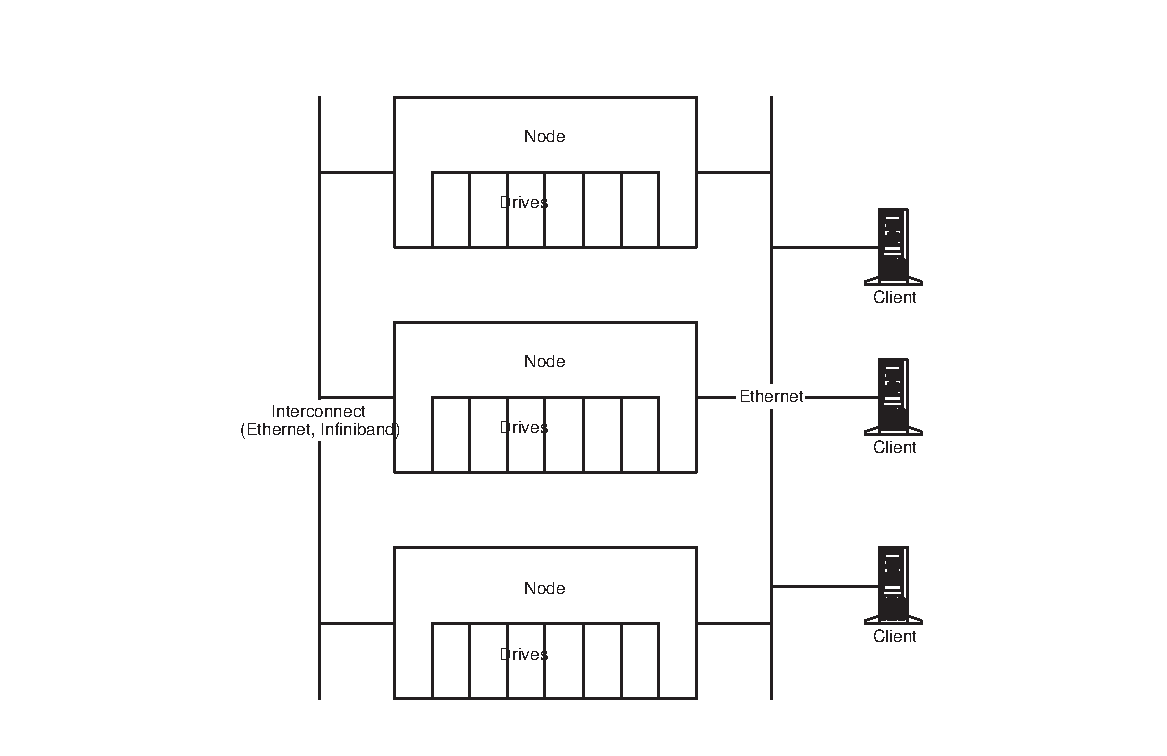
\includegraphics[width=\textwidth]{ClusterDiagram}
\end{center}
\caption{NAS Clustered Storage System}
\label{fig-nas-cluster}
\end{figure}

\subsection{Redundancy}
\label{sec-redundancy}

Redundancy forms the basis for claims of clustered storage system reliability.
The basic idea is identical to that used for RAID.  A $k$-out-of-$n$ system
can be built from $n$ components by storing redundancy information.

The simplest approach to redundancy is to use mirroring.  Multiple components
store an identical copy of a piece of data.  If any given copy becomes lost or
unavailable, the remaining copies may still be accessed.  If the mirroring
level is $n$, then mirroring provides a 1-out-of-n system.

Although mirroring is simple, it creates significant storage overhead.  In the
common case, redundant information is not accessed.  There are much more
efficient schemes which require extra work to rebuild and calculate the
redundancy information.  Such schemes employ {\em error-correcting codes} to
create redundancy.  With error-correcting codes, the overhead of redundancy
can be reduced.  For $n$ data units, these schemes can create $m$ additional
units of data, such when units are lost, any $n$ of the $n+m$ units can be
used to reconstruct the data.  This yields a $n$-out-of-$n+m$ system, where
$m$ can be increased to improve reliability, at the cost of calculation
overhead and additional space.  A good reference for the engineer can be
found in \cite{plank}.  

In this system model, redundancy information is striped across nodes.  Data is
broken up into {\em stripes} which contain some range of the data and the
redundancy information for that data.  The redundancy level is characterized
by $m$, which is the number of failures which can be tolerated without data
loss.  The stripes are of size $n+m$, and require $n+m$ distinct nodes.  For
example, to protect data at $6+3$, nine nodes are required.  This results in
the redundancy information adding 50\% overhead.

These redundancy sets are not partitioned.  If data is protected at $8+2$ on a
system with 20 nodes and two nodes fail, there may exist a redundancy set
which includes both those nodes.  The only limit to the redundancy sets is
that each unit must be stored on a separate node.  Thus, drives within the
same node never share a redundancy set unless they store information for the
same unit.

\subsection{Failure as Data Loss}

There are a number of ways to interpret the reliability of a storage system
since ``failure'' can be defined quite broadly.  A storage system can fail for
all the same reasons as any complex computer system.  For this work, we want
to capture the critical failures while keeping the problem tractable.  
Since the main purpose of a storage system is to store data, we will define
failure as file system {\em data loss} due to failed storage components. 

Data loss occurs when enough components stop functioning that data stored in
the file system becomes unrecoverable, that is, when more than $m$ components
in a $n+m$ redundancy set fail.  When any component fails, a repair process
must be started to restore the redundancy.  In the following sections,
component failures and the process of repair are defined.

\subsection{Component Failures}

A clustered storage system is composed of many independent hardware
components, including drives, CPUs, interconnect, and cooling fans.
Enumerating all component failure rates is beyond the scope of this paper.
Some simplification is required.  In this paper, node and drive failures are
the focus.

\subsubsection{Drives}

Drives are the most numerous logically separable component in the system.  A
single node may have anywhere from 8 to hundreds of drives.  Drives are the
most important component of the system since they are the stable storage for
the data; when they are lost data is lost.  Drives are also one of the least
reliable components owing to their rotating mechanical assembly and delicate
magnetic media.  

Drive manufacturers usually quote MTTFs in the range of hundreds of thousands
of hours.  These numbers assume replacement before the wear-out period.  It's
important to note that this document assumes replacement at the manufacturer's
recommended time period.

Drive reliability is a rich subject which is highly dependent upon the data
made available by manufacturers.  There are multiple classes of drives with
varying levels of cost, performance, and reliability.  The reader is
encouraged to investigate this subject separately.  In the context of this
paper drives are assumed to have a failure rate of approximately 1\% per year.

\subsubsection{Nodes}

Node failure captures the failure of all the other components of the system.
These components are similar to any personal computer system:  CPU, fans,
power supply, motherboard, NICs, and more.  With the exception of the fans,
most of these components are solid-state and therefore usually more reliable
than drives.  

Also, these components are not responsible for the stable storage of data, and
therefore can typically be replaced without losing data.  In the context of
this paper, the node failure rate is intended to capture all the components
which require replacement of the node.  Field-replaceable node sub-components
typically impact availability of the data on the enclosed drives, but not the
reliability.

In practice, it may be possible to preserve drive data, even when a node must
be replaced.  This reduces the effective node failure rate to be the failure
rate of components which impact drive integrity.  This effect is not addressed
in this paper.

\subsection{Repair}
\label{sec-repair}

When a component fails, file system data can be rebuilt using the remaining
space in the cluster.  The process of repair is generally scalable; more nodes
in the cluster provides more system throughput for rebuilding data.  This
repair process typically completes in a matter of hours.  This is faster than
traditional storage architectures since all the hardware in the cluster is
employed to effect the repair.

The process of repair restores the specified level of redundancy.  At some
later point, the failed component may be replaced with a new unit.  For
drives, this has little effect on the system.  For nodes, the effect can be
more dramatic since so much space must be used to store information from the
failed node.  In practice, the process of repair would need to wait for node
replacement before rebuilding the redundancy, but this effect is ignored here.

%%%%%%%%%%%%%%%%%%%%%%%%%%%%%%%%%%%%%%%%%%%%%%%%%%%%%%%%%%%%%%%%%%%%%%%%%
\section{Methodology}
\label{sec-methodology}

Evaluating the reliability of a repairable system is a complex task.  It
depends on a number of assumptions which may significantly effect the outcome.
This section introduces the concepts, notations, and assumptions which
characterize the analysis.

\subsection{Reliability Concepts}

The reliability function for a system, denoted by $R(t)$, indicates the
probability of the system functioning at time $t$.  The failure distribution
function is denoted by $f(t)$, and represents the p.d.f. for $t$.  Evaluating
the reliability of a system typically means characterizing $R(t)$ (or $f(t)$
since there is a known relationship).

In most contexts, it is convenient to characterize the reliability of a system
with a single number, rather than a distribution function.  The typical number
presented is the expected value of $f(t)$, which is the average, or mean,
value of $t$.  This is often referred to as the mean time to failure (MTTF).
For system with perfect repair, MTTF is the same as the mean time between
failures (MTBF).  

Although it is convenient for the layman, characterizing the reliability using
the MTTF can be misleading.  For example, people frequently expect that
$R(MTTF) = 0.5$.  That is, that the mean is also the median.  This is highly
dependent on $f(t)$.  For example, for the normal distribution, the mean is
equal to the median, but for the exponential distribution, the mean represents
the $63.2$ percentile.  Depending on the context it may be more effective to
characterize the reliability in terms of the $10^{th}$ percentile or
reliability at some time $t$, such as five years.

This paper assumes a constant failure rate.  With a constant failure rate,
$f(t)$ is an {\em exponential distribution}, shown by $f(t) = \lambda
e^{-\lambda t}$.  This allows a single parameter, $\lambda$, the failure rate,
to characterize the reliability.  Since $\lambda = 1/\textrm{E[$t$]}$,
converting between the failure rate and mean is easy.  The rest of the paper
will be concerned with characterizing the reliability with the MTTF of the
system.

\subsection{Notations}

The literature on this subject frequently presents a variety of notations, and
this system in particular must be characterized by certain parameters.  Below
are the mathematical notations that will be used throughout the document.  
\\

\begin{tabular}{ll}
$G$ & RAID group size 
\\
$m$ & Redundancy level, or number of failures that can be tolerated 
\\
$d$ & The number of drives per node 
\\
$N$ & The number of nodes in the cluster 
\\
$\lambda_{d}$ & The failure rate of drives 
\\
$\lambda_{N}$ & The failure rate of nodes 
\\
$\mu_{d}$ & Drive repair rate
\\
$\mu_{N}$ & Node repair rate
\end{tabular}

\subsection{Failure Model}

In order to characterize system reliability, the reliability of the individual
components must be characterized.  The failure rate of electronic components
is typically characterized by a "bathtub curve".  In this model, the initial
failure rate is high due to manufacturing defects.  This is followed by a
period of constant failure rate representing the inherent reliability of the
product.  A time goes by the product suffers wear-out and the failure rate
starts to increase.

Organizations try to avoid the higher failure rates at the ends of the bathtub
curve, which can prove disastrous for system reliability.  The birth end of
the curve is typically addressed by a "burn-in" process which attempts to
trigger failures due to manufacturing defects.  The wear-out period is avoided
by limiting the warranty or providing some incentive for replacement.

For this paper, the failure rate is assumed constant.  This is reasonable for
a clustered storage system since the ends of the bathtub curve are relatively
easy to avoid.  For burn-in, the system can be given simulated load for
24-48hrs on-site via built-in software.  In addition to catching manufacturing
defects, this process also finds problems in shipping.  Wear-out is less of a
concern since computer systems become obsolete quickly.  Furthermore, with much
of the complexity in software, the hardware is relatively cheap to replace.

The failure model being used here also assumes that failures are detected.
This is referred to as {\em fail-stop} behavior, since the failed device
stops performing its function.  This is in contrast to ``Byzantine" failures,
where devices may produce any possible output.  Byzantine fault-tolerance is
considered beyond the scope of this work, and is typically not a significant
concern in systems such as the one under consideration.

When characterizing the reliability of the clustered storage system, the MTTF
of the system will be described as mean time to data loss (MTTDL), to help
distinguish it form individual component MTTFs.

\subsection{General Assumptions}

Any complex analysis relies on a simplifying set of assumptions.  This
sections lists the assumptions made here, along with some justification.

\begin{itemize}
  \item {\em Component failure is detectable.}  
  This is mentioned in the previous section.  In this clustered storage model,
  component failures are not allowed to cause arbitrary behavior (called {\em
  Byzantine failure}).  In practice, it is rare for devices to exhibit true
  Byzantine failure, though there is some measurable chance of devices
  introducing single bit errors.  These bit errors can be converted into
  detectable errors using checksums, or detected and corrected using
  error-correcting codes.

  \item {\em Failures are i.i.d.} 
  This is not the case for several reasons.  The failure of one component
  causes a repair process to start which increases load on the remaining
  components.  Hard drives in particular tend to be vulnerable to
  environmental factors, which represent a common cause (covered in the next
  section).

  \item {\em Repair time is constant}.  
  Repair time is determined by a number of installation-specific
  characteristics, including load, cluster size, and space used.  Repair time
  is probably better modeled as a log normal distribution.  Instantaneous
  repair is very unlikely; there is a band of high probability based on the
  number of nodes, size of drives, and hardware performance; finally, there is
  a long tail representing all the various unlikely conditions that may delay
  repair.  For this analysis, we assume that in practice,
  installation-specific parameters can be incorporated by using observed repair
  times, since any reasonably large installation will have an all-component
  MTBF on the order of months.

  \item {\em Repair is perfect}.  
  In this clustered storage system model, failed components are replaced with
  new components.  These standby components suffer no degradation, and are
  assumed equivalent to other components in the system.  In practice, standby
  components may not be identical, since computer system components become
  obsolete so fast.
\end{itemize}

\subsection{Ignored Factors}

Some behaviors of this clustered storage system are difficult to quantify or
require analysis beyond the scope of this document.  In any reliability
analysis, it's important to identify which factors are {\em not} being
considered so that estimates can be properly qualified. 

The following factors are ignored in this paper, though there may be
significant research into quantifying the effects.  The reader is encouraged
to research these topics separately.

\begin{itemize}
    \item {\em Disk sector failures}.
    Healthy disk drives sometimes report individual sector read failures.
    This can cause data loss of just the sector, which is just 512B, or could
    make the file system unusable if the sector holds crucial metadata.

    \item {\em Environmental Problems}.
    Environmental problems are a ``common cause'' that can cause multiple
    nodes to fail.  This violates the independence of component failures.
    This is mostly outside the system designer's control, but is an important
    consideration for any organization.

    \item {\em User error}.
    Issues such as misconfiguration, improper maintenance and vandalism are
    legitimate threats to reliability of any system.  These threats are highly
    dependent on the implementation and generally difficult to quantify.

    \item {\em Software defects}.
    Software problems can cause a clustered storage system to fail.  The file
    system may become corrupt, or some critical functionality may stop
    working.  The effects of software defects are highly dependent upon the
    implementation.  There is significant research on this subject.  

    \item {\em Partial Repair}.
    With double redundancy, it's possible for a component to fail during the
    repair of another component.

    \item {\em Physical replacement delay}.
    In this clustered storage model, all the space in the system can be used
    to repair the loss of a component, so no physical replacement or standby
    component is required to effect repair.  However, any reasonably utilized
    system will quickly run out of space without replacement.  It's assumed
    here that the replacement interval is much less than the overall failure
    rate of components.
\end{itemize}

%%%%%%%%%%%%%%%%%%%%%%%%%%%%%%%%%%%%%%%%%%%%%%%%%%%%%%%%%%%%%%%%%%%%%%%%%
\section{Approaches to Evaluating Repairable $k$-out-of-$n$ Systems}

Evaluating the reliability of a non-repairable $k$-out-of-$n$:G system with
identical components can be straightforward.  When replacement is not
considered at all, the reliability can be easily expressed as the probability
of more than $k$ components functioning:
$$r(k, n) = \sum_{i=k}^{n} {n \choose i} R^{i}(1 - R)^{n - i}$$
When the system contains multiple component types, and components may be
repaired, the system reliability is not as easy to evaluate.  This section
presents three basic approaches to evaluating such a system.

\subsection{Direct Analysis}

Most approaches to analyzing system reliability involve enumerating the various
combinations of failures and evaluating the individual probabilities.  This
quickly becomes intractable for a system with several components, and
especially so in the context of clustered storage where literally thousands of
hard drives may be involved.  Since many of the components are identical,
there can be some simplification, but direct analysis remains difficult.  In
this paper, direct analysis of a simple RAID system is presented in
section~\ref{sec-raid}, which is the only analysis of this form presented.

\subsection{Markov Analysis}

Complex systems may be difficult to evaluate by enumerating the various
combinations of failures.  Sometimes it is easier to look at particular states
and the transitions between them.  This approach is referred to as Markov
analysis.

A {\em Markov process} is random process wherein the transition between states
only depends on the current state.  If $I$ is the set of states, then a given
state $i$ has some probability $p_{ij}$ of transitioning to each state $j$ in
$I$.  A Markov state diagram shows the possible states and their transitions.

For example, consider a discrete system with two states, $1$ and $2$.  The
system transitions between states in a series of discrete steps.  In state,
$1$, there is a probability $1/2$ of transitioning to state $2$, and similarly
and probability $1/4$ of transitioning to state $1$ from state $2$.  Then the
stochastic probability matrix for this system is:

\begin{displaymath}
\mathbf{P} =
\left( \begin{array}{cc}
1/2 & 1/2 \\
1/4 & 3/4 \\
\end{array} \right)
\end{displaymath}

This matrix form allows for use of linear algebra methods in evaluating
statistical properties.  This example was a case of a discrete Markov chain,
where transitions occur in a series of steps.  For repairable system
reliability we are concerned with time as a continuous value, but the same
principles will apply.  For further general discussion of Markov chains
methods see \cite{chains}.

\subsection{Monte Carlo Simulation}

Probalistic analysis of a repairable $k$-out-of-$n$ grows ever more complex as
new components and behaviors are included.  State transitions may no longer
have the Markov property.  For some combinations of failure distributions and
components, a closed-form solution for the MTTDL may not even be possible.

Monte Carlo simulation is well suited for more complex systems.  The
reliability engineer is free to incorporate any number of states and any
interactions between components.  Furthermore, any properties of the random
variable can be recorded without having to perform new analysis.

\subsubsection{Theoretical Basis}

Let $\mathbf{X} = (X_{1}, \ldots, X_{n})$ denote a random vector having a
given density function $f(x_{1}, \ldots, x_{n})$ and suppose we are interested
in determining the expected value of a function $g(\mathbf{X})$.  Suppose it
is not analytically possible to compute or even approximate the expectation.

One way of approximating $E[g(\mathbf{X})]$ is by simulation.  Generate a
$\mathbf{X}_{i}$ and compute $Y_{i} = g(\mathbf{X}_{i})$.  Do this $r$ times,
and by the strong law of large numbers, $$\lim_{r \to \infty} \frac{\sum
Y_{i}}{r} = E[Y_{i}] = E[g(\mathbf{X})]$$
    
Central to Monte Carlo simulation is the ability to simulate a random variable
with a specific distribution.  In this case, the lifetime of drives is often
assumed to be an exponential distribution, yet we generally think of producing
uniformly distributed random variables.  To produce a random variable with a
given continuous distribution from a uniform random variable, we use the
following proposition as defined in \cite{prob}:

\begin{quote} 
Let $U$ be a uniform $(0,1)$ random variable.  For any continuous distribution
function $F$, if we define the random variable $X$ by $$X = F^{-1}(U)$$ then
the random variable $X$ has distribution function $F$.
\end{quote}

We can employ Monte Carlo simulation by letting $g(x)$ be the failure p.d.f.
for the time to data loss.  Then,
$$\textrm{MTTDL} = E[f(\mathbf{T}_{DL})]$$

\subsubsection{Implementation}

A Monte Carlo simulator for this clustered storage system is similar to many
event-based simulations.  Future events are generated randomly.  The
simulation moves forward to the next event in time, effects that event in the
simulated objects, and generates more events.  The simulation
may end after a period of time, or for this application, at system failure.

\begin{figure}[h]
\begin{center}
\end{center}
\begin{verbatim}
for each component:
    queue.insert(random_failure(component))
while true:
    event = queue.pop()
    if is_failure(event):
        if data_loss:
            break
        else:
            queue.insert(repair(event.component))
    if is_repair(event):
        queue.insert(random_failure(event.component)
\end{verbatim}
\caption{Psuedo-code for Monte Carlo simulation}
\label{fig-monte-carlo}
\end{figure}


Figure \ref{fig-monte-carlo} shows psuedo-code for a Monte Carlo simulation of
the clustered storage system under consideration.  This algorithm produces one
sample for $t_{DL}$.  This algorithm can be run multiple times and averaged to
produce the MTTDL.  Additional statistical properties of $t_{DL}$ can also be
generated from these samples, such as variance or percentiles. 

Choosing an appropriate number of runs can be difficult.  One approach is to
specify a precision and run simulations until the desired precision is
reached.  This can be accomplished using the relatively uncertainty in the
parameter, which is:

$$\frac{\sigma}{\bar{t}\sqrt{n}}$$

where $\sigma$ is the standard deviation, $\bar{t}$ is the expected value of
$t$, and $n$ is the number of iterations.  This is explained in \cite{eval}.
This simulator was implemented and will be used to provide independent
verification of Markov analysis.

%%%%%%%%%%%%%%%%%%%%%%%%%%%%%%%%%%%%%%%%%%%%%%%%%%%%%%%%%%%%%%%%%%%%%%%%%
\section{RAID Reliability}
\label{sec-raid}

As RAID systems are the basis for clustered storage, the reliability of RAID
systems also forms the basis for clustered storage reliability.
Section~\ref{sec-cluster} will then apply these results to evaluate the
reliability in limited cases, and thus validate more complete results.

In the context of this section, a RAID system is a group of $G$ disks with
some amount of redundancy $m$, where $m+1$ failed disks within the group
indicate data loss.  RAID systems are typically implemented with 8-16 disks,
where the redundancy stripes range from 7+1 to 14+2.

\subsection{Direct Analysis}

Using direct analysis we can calculate the ${\rm MTTDL_{+1}}$.  Note that if
we assume data loss is exponentially distributed, then this single parameter
is sufficient to characterize the reliability of the system.  Since there is
no time-dependency in the calculation, data loss is assumed to be
exponentially distributed.

The following argument is presented in \cite{raid}.  It is reproduced here
using this paper's notation and extended for additional redundancy levels.
Let $G$ be the number of disks in the redundancy set.  We first assume
independent and exponential failure rates.  This model uses a biased coin with
the probability of heads being the probability that a second failure will
occur with the MTTR of a first failure.  Since disk failures are exponential,

\begin{eqnarray}
\textrm{P(failure during repair)} & = & 1 - \prob{no failures during repair} 
\\
& = & 
1 - R_{1}(1/\mu_{d}) R_{2}(1/\mu_{d}) \cdots R_{G-1}(1/\mu_{d})
\\
& = & 
1 - R_{d}(1/\mu_{d})^{G - 1}
\\
& = & 1 - (e^{-\lambda_{d}/\mu_{d}})^{G-1} 
\end{eqnarray}

In any practical scenario,

$$\mu_{d} \gg \lambda_{d} \cdot G$$

and since $(1 - e^{-x}) \approx x$ for $0 < x \ll 1$


$$\textrm{P(failure during repair)} = \frac{\lambda_{d}\cdot (G-1)}{\mu_{d}}$$

Then that on a disk failure we flip this coin
\begin{itemize}
\item[] heads $\Rightarrow$ a system crash, because a second failure occurs
before the first was repaired.
\item[] tails $\Rightarrow$ recover from error and continue.
\end{itemize}

Then,

\begin{eqnarray}
{\rm MTTDL_{+1}} & = & \textrm{E[Time between failures]} \cdot 
\textrm{E[flips until heads]} 
\\
& = & \frac{\textrm{E[Time between failures]}}{\textrm{P(heads)}} 
\\
& = & \frac{1}{\lambda_{d} \cdot G} \cdot 
\frac{\mu_{d}}{\lambda_{d} (G-1)} 
\\
& = & \frac{\mu_{d}}{G \cdot (G-1) \cdot \lambda_{d}^{2}} 
\end{eqnarray}

This addresses the case of +1 redundancy, that is tolerating one failure.  What
happens if we add arbitrary redundancy?  Fortunately, there is a
straightforward way to extend this same argument.  

For our +1 analysis, we started with the MTBF of drive failures, and then
considered the number of failures which occur before a second failure occurs
during the repair.  For the general case, we start with the frequency of $m$
simultaneous failures, and consider the number of such cases which occur until
there is data loss.

\begin{eqnarray}
{\rm MTTDL_{m+1}} & = & \textrm{E[Time between $m$ failures]} \cdot 
\textrm{E[flips until heads]} 
\\
& = & \frac{\textrm{E[Time between $m$ failures]}}{\textrm{P(heads)}} 
\\
& = & {\rm MTTDL_{m}} \cdot \frac{\mu_{d}}{\lambda_{d} (G-(m+1))} 
\end{eqnarray}

Thus, we can construct the MTTDL for $m$ redundancy:
\begin{eqnarray}
{\rm MTTDL_{m}} & = & \frac{1}{\lambda_{d} \cdot G} \cdot 
\frac{\mu_{d}}{\lambda_{d} (G-1)} \cdots \frac{\mu_{d}}{\lambda_{d} (G-m)} \\
& = & \frac{\mu_{d}^{m}}{\displaystyle \prod_{i=0}^{m}(G - i)\lambda_{d}^{m+1}} 
\label{eq-raid}. 
\end{eqnarray}

\subsection{Markov Analysis}
\label{sec-raid-markov}

We now apply Markov analysis to RAID storage systems.  For $m=1$, there are
three basic states: no failures, one failure, and data loss.
Figure~\ref{fig-markov-raid} shows the state diagram, with these three states
numbered 1, 2, and 3, respectively.  State 3, data loss, is an {\em absorbing
state} since the system has failed and cannot be repaired.

\begin{figure}[h]
\begin{center}
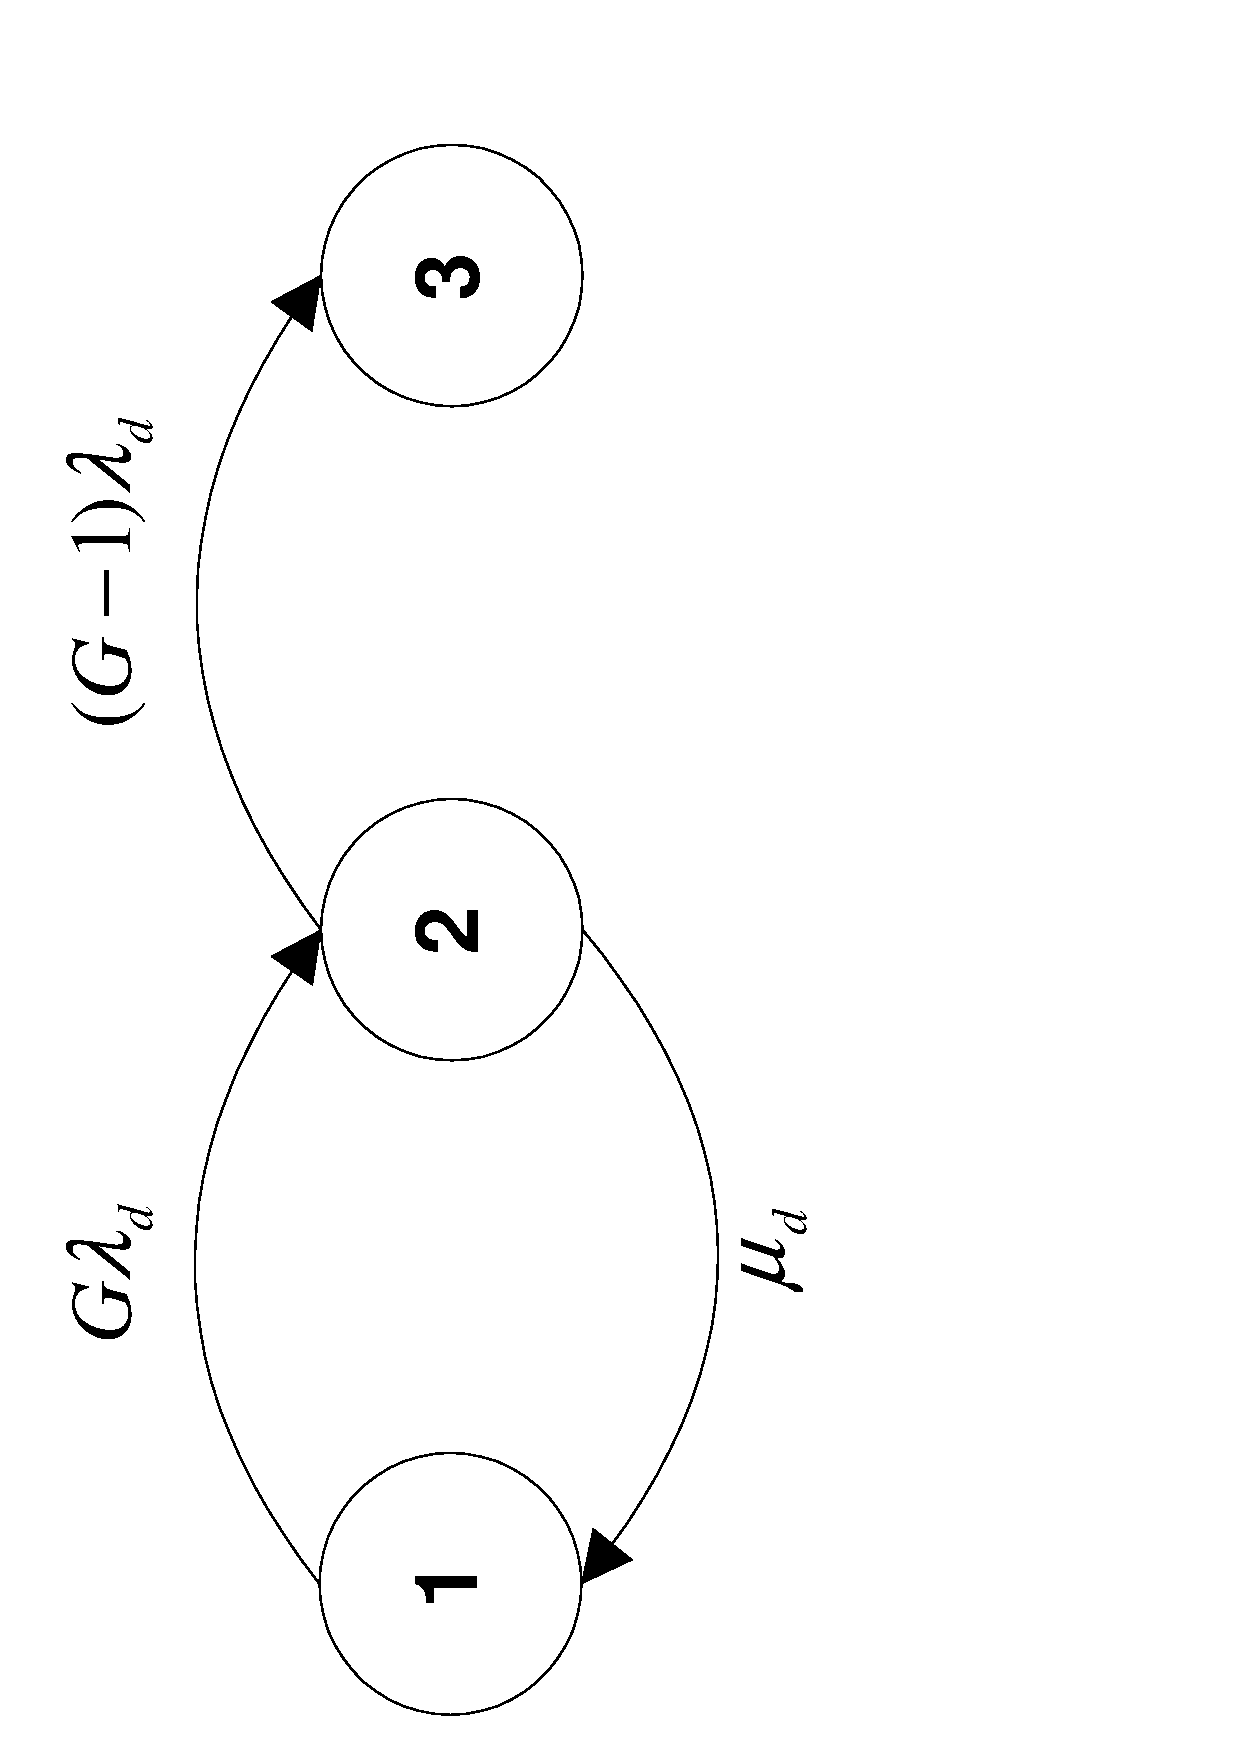
\includegraphics[angle=270,width=0.5\textwidth]{DriveMarkov}
\end{center}
\caption{Markov Model for RAID with +1 redundancy}
\label{fig-markov-raid}
\end{figure}

The stochastic transitional probability matrix (with $\Delta t$ omitted) is:
\begin{displaymath}
\mathbf{P} =
\left( \begin{array}{ccc}
1 - G \lambda_{d} &  G \lambda_{d} &  0  \\
\mu_{d}           & 1 -  (G - 1)\lambda_{d} - \mu_{d}  & (G - 1)\lambda_{d} \\
0                 &  0  & 1              \\
\end{array} \right)
\end{displaymath}

We are primarily concerned with the MTTDL, so we use the method outlined in
\cite{eval} to calculate it from the probability matrix.  First, we create the
truncated matrix $\mathbf{Q}$ to account for the absorbing data loss state.

\begin{displaymath}
\mathbf{Q} =
\left( \begin{array}{cc}
1 - G \lambda_{d} &  G \lambda_{d}  \\
\mu_{d}           & 1 -  (G - 1)\lambda_{d} - \mu_{d}  \\
\end{array} \right)
\end{displaymath}

Next, we calculate the matrix $\mathbf{M}$, in which each element $m_{ij}$
represents the time spent in state $j$ given the process starts in state $i$.

\begin{eqnarray}
\mathbf{M} & = & (\mathbf{I} - \mathbf{Q})^{-1} \\
& = & \left( 
\left( \begin{array}{cc}
1 & 0 \\
0 & 1 \\
\end{array} \right) - 
\left( \begin{array}{cc}
1 - G \lambda_{d} &  G \lambda_{d}  \\
\mu_{d}           & 1 -  (G - 1)\lambda_{d} - \mu_{d}  \\
\end{array} \right)
\right)^{-1} 
\\
& = & 
\left( \begin{array}{cc}
G \lambda_{d} &  - G \lambda_{d}  \\
- \mu_{d}     & (G - 1)\lambda_{d} + \mu_{d}  \\
\end{array} \right)^{-1} 
\\
& = & 
\frac{1}
{G (G - 1)\lambda_{d}^{2}}
\left( \begin{array}{cc}
(G - 1)\lambda_{d} + \mu_{d} &  G \lambda_{d}  \\
\mu_{d}     & G \lambda_{d}  \\
\end{array} \right)
\end{eqnarray}

Finally, since we only care about cases where the system starts in state 1,

\begin{eqnarray}
\mttdl & = & 
\frac{(G - 1)\lambda_{d} + \mu_{d} + G \lambda_{d}}
{G (G - 1)\lambda_{d}^{2}} 
\\
& = & 
\frac{\mu_{d}}{G (G - 1)\lambda_{d}^{2}} + 
\frac{(G - 1)\lambda_{d}}{G (G - 1)\lambda_{d}^{2}} + 
\frac{G \lambda_{d}}{G (G - 1)\lambda_{d}^{2}} 
\\
& = & 
\frac{\mu_{d}}{G (G - 1)\lambda_{d}^{2}} + 
\frac{1}{G \lambda_{d}} + 
\frac{1}{(G - 1)\lambda_{d}} 
\end{eqnarray}

The similarity to equation (\ref{eq-raid}) is clear, though additional
terms result from the simplifying assumptions made in section \ref{sec-raid}.

%%%%%%%%%%%%%%%%%%%%%%%%%%%%%%%%%%%%%%%%%%%%%%%%%%%%%%%%%%%%%%%%%%%%%%%%%
\section{Clustered Storage Reliability}
\label{sec-cluster}

The previous section explained how the reliability of a RAID system may be
evaluated.  Now we consider the reliability of our clustered storage system.
First, the RAID equation for MTTDL is applied to nodes and drives separately.
Then the combined result is presented based on Markov analysis.  These
results can be compared to the combined result when $\lambda_{d}=0$ and
$\lambda_{N}=0$, respectively.

\subsection{Applying RAID Reliability}

First we consider only node failures.  In this case, each nodes behaves
exactly like a drive in a RAID system.  Since the redundancy information is
not partitioned, the failure of any $m+1$ nodes can cause data loss.  Thus,
the raid group size $G$ is the number of nodes $N$, and we replace the drive
failure and repair rates in equation \ref{eq-raid} with those of nodes: 

\begin{equation}
\mttdl = \frac{\mu_{N}^{m}}{\displaystyle \prod_{i=0}^{m}(N -
i)\lambda_{N}^{m+1}}
\label{eq-raid-nodes}
\end{equation}

Since there are typically several drives per node, and drives tend to be the
more unreliable components by design, a node-only MTTDL is not very useful.
Fortunately, the RAID MTTDL equation can be modified to only account for 
drives in the cluster storage system.

Most drives in the clustered storage system are potentially part of the same
redundancy set.  Since data is striped across nodes, drives in the same node
are {\em not} in the same redundancy set.  That is, multiple drive failures
within a node still only count as one failure against the redundancy level of
the data ($m$).

Thus, during repair, only a failure in the nodes outside of those already
having a failure can cause data loss.  At each failure, the number of nodes
which may cause a critical failure are reduced.

\begin{eqnarray}
\mttdl & = & 
\frac{1}{\lambda_{d} \cdot N \cdot d} \cdot 
\frac{\mu_{d}}{\lambda_{d} (N-1)d} \cdots \frac{\mu_{d}}{\lambda_{d} (N-m)d} 
\\
& = & \frac{\mu_{d}^{m}}
{\displaystyle \prod_{i=0}^{m}(N - i)d^{m+1}\lambda_{d}^{m+1}}
\label{eq-raid-drives}
\end{eqnarray}

\subsection{Combined Reliability Model}

A Markov analysis of similar storage systems is presented in \cite{ibm}.  A
simplified version is shown in figure~\ref{fig-markov-cluster}.  The diagram
is constructed by increasing the number of drive failures along the x-axis of
the diagram and increasing the number of node failures along the y-axis of the
diagram.  The absorbing state, data loss, is indicated by state F and occurs
when $m+1$ nodes are either failed or have a drive failed.

Solving for the MTTDL using matrix methods is beyond the scope of this
document.  As shown in \cite{ibm}, this matrix yields the following result:

\begin{equation}
\mttdl = \frac{(\mu_{d}\mu_{N})^{m}}
{\displaystyle \prod_{i=0}^{m} 
(N - i)(\lambda_{N} + d\lambda_{d})
(\mu_{d}\lambda_{N} + d\mu_{N}\lambda_{d})^{m}}
\label{eq-combined}
\end{equation}

If this is correct, then it should match equations (\ref{eq-raid-nodes}) and
(\ref{eq-raid-drives}) when drive and node failures are ignored, respectively.

First, let us ignore drive failures.  Then, $\lambda_{d} = 0$, and equation
(\ref{eq-combined}) becomes:

\begin{eqnarray}
\mttdl & = & \frac{(\mu_{d}\mu_{N})^{m}}
{\displaystyle \prod_{i=0}^{m} 
(N - i)(\lambda_{N} + d\cdot 0)
(\mu_{d}\lambda_{N} + d \mu_{N} \cdot 0)^{m}}
\\
& = & \frac{\mu_{d}^{m}\mu_{N}^{m}}
{\displaystyle \prod_{i=0}^{m} 
(N - i)
\mu_{d}^{m}\lambda_{N}^{m+1}}
\\
& = & \frac{\mu_{N}^{m}}
{\displaystyle \prod_{i=0}^{m} 
(N - i)
\lambda_{N}^{m+1}}
\end{eqnarray}

This shows that equation (\ref{eq-combined}) matches (\ref{eq-raid-nodes})
when drive failures are ignored.  Now let us ignore node failures, such that
$\lambda_{N} = 0$.  Then, equation (\ref{eq-combined}) becomes:

\begin{eqnarray}
\mttdl & = & \frac{(\mu_{d}\mu_{N})^{m}}
{\displaystyle \prod_{i=0}^{m} 
(N - i)(0 + d\lambda_{d})
(\mu_{d}\cdot 0 + d \mu_{N} \lambda_{d})^{m}}
\\
& = & \frac{\mu_{d}^{m}\mu_{N}^{m}}
{\displaystyle \prod_{i=0}^{m} 
(N - i)d^{m+1}
\mu_{N}^{m} \lambda_{d}^{m+1}}
\\
& = & \frac{\mu_{d}^{m}}
{\displaystyle \prod_{i=0}^{m} 
(N - i)d^{m+1} \lambda_{d}^{m+1}}
\\
\end{eqnarray}

Now we see that (\ref{eq-combined}) is equivalent to (\ref{eq-raid-drives})
when node failures are ignored.  

Hence, as we would expect, the Markov analysis is consistent with the direct
analysis of the MTTDL.  While it is reassuring that two distinct methods
produced consistent results, these two approaches rely on similar principles.
In the next section, we determine whether equation (\ref{eq-combined}) is
consistent with results from Monte Carlo simulation.

%%%%%%%%%%%%%%%%%%%%%%%%%%%%%%%%%%%%%%%%%%%%%%%%%%%%%%%%%%%%%%%%%%%%%%%%%
\section{Verification}

Since this paper evaluates the reliability of an abstract clustered storage
system model, there is no field data to validate the MTTDL estimates.  The
Markov analysis has been validated against the direct analysis of RAID
reliability for limited cases.  This section compares specific results from
simulation to the Markov analysis to provide some confidence in this analysis.
All the assumptions and simplifications are shared between the simulation and
the analytic approaches.  Thus, there is no validation of those assumption and
simplifications.

Figure \ref{fig-results} lists the MTTDL of select scenarios as calculated by
both the equation (\ref{eq-combined}) and Monte Carlo simulation.  The numbers
are chosen to be reasonable real-world values and provide reasonable coverage
of the input space.

\begin{figure}[h]
\begin{center}
\begin{tabular}{|rrrrrrr|r|r|}
\hline
& & $1/\lambda_{N}$ & $1/\lambda_{d}$ & $1/\mu_{N}$ & $1/\mu_{d}$ &  & 
\multicolumn{2}{c|}{MTTDL (years)}
\\
$N$ & $d$ & (years) & (years) & (hours) & (hours) & $m$ &
Simulation & Equation 
\\
\hline
10 & 8  & 150 & 75 & 48 & 8 &  1 & 754 &  731 
\\
\hline
10 & 16 & 150 & 75 & 24 & 6 &  1 & 316 & 307
\\
\hline
20 & 12 & 50 & 50  &  36 & 10 &  2 &  3015 & 4432 
\\
\hline
20 & 24 & 50 & 50  & 30 & 5 &  2 &  1435 & 2493  
\\
\hline
100 & 16 & 100 & 100 & 40  & 9  &  3 & 1836 & 6744
\\
\hline
100 & 32 & 100 & 100 & 30  & 7 &  3 & 534 & 1321 
\\
\hline
\end{tabular}
\end{center}
\caption{MTTDL estimates from simulation and equation (\ref{eq-combined})}
\label{fig-results}
\end{figure}

The results are mixed.  When $m=1$, the estimates are quite close.  The
results for $m=2$ and $m=3$, are off by a factor of 2 and 3 respectively.
Given the scale of the values, that is, the polynomial impact of $m$, the
values are close enough to validate both approaches.  There appears to be some
relatively subtle difference which grows with $m$.

One possible explanation is a difference in the way the simulator and Markov
model treat repair under multiple failures.  With the Markov model, when
repair is interrupted, the system ``forgets'' any progress made on rebuilding
data on existing failed components, and considers all failures to have
occurred concurrently.  In the simulator, further failures don't adjust the
repair time of existing failed components, which more closely matches a real
system.  This effect is negligible when $m=1$ because additional failures
during repair cause data loss.  The effect is multiple with larger values of
$m$ because repair can be interrupted multiple times by further failures.

Furthermore, neither model accounts well for multiple drive failures on the
same node.  In the Markov analysis, this effect is completely ignored.  In the
simulator, drive failures in the same node have the same repair time.  But
the failure of one drive loads the system such that additional failures slow
the repair rate of each failure.

%%%%%%%%%%%%%%%%%%%%%%%%%%%%%%%%%%%%%%%%%%%%%%%%%%%%%%%%%%%%%%%%%%%%%%%%%
\section{Conclusion and Future Work}

This document has surveyed methods of evaluating the reliability of a
clustered storage system.  Repairable $k$-out-of-$n$ systems are a challenge
for system reliability analysis. Two main approaches, Markov Analysis and
Monte Carlo simulation were introduced and compared.  These methods were
validated with some limited success.  

Future work will need to include refining both approaches and using field data
of a particular system to validate the models.  The repair process appears to
be a challenge in all cases, since certain subtleties of repair are difficult
to model.  The most important goal, however, is to treat repair consistently
so that results can be fairly compared.

\begin{figure}[h]
\begin{center}
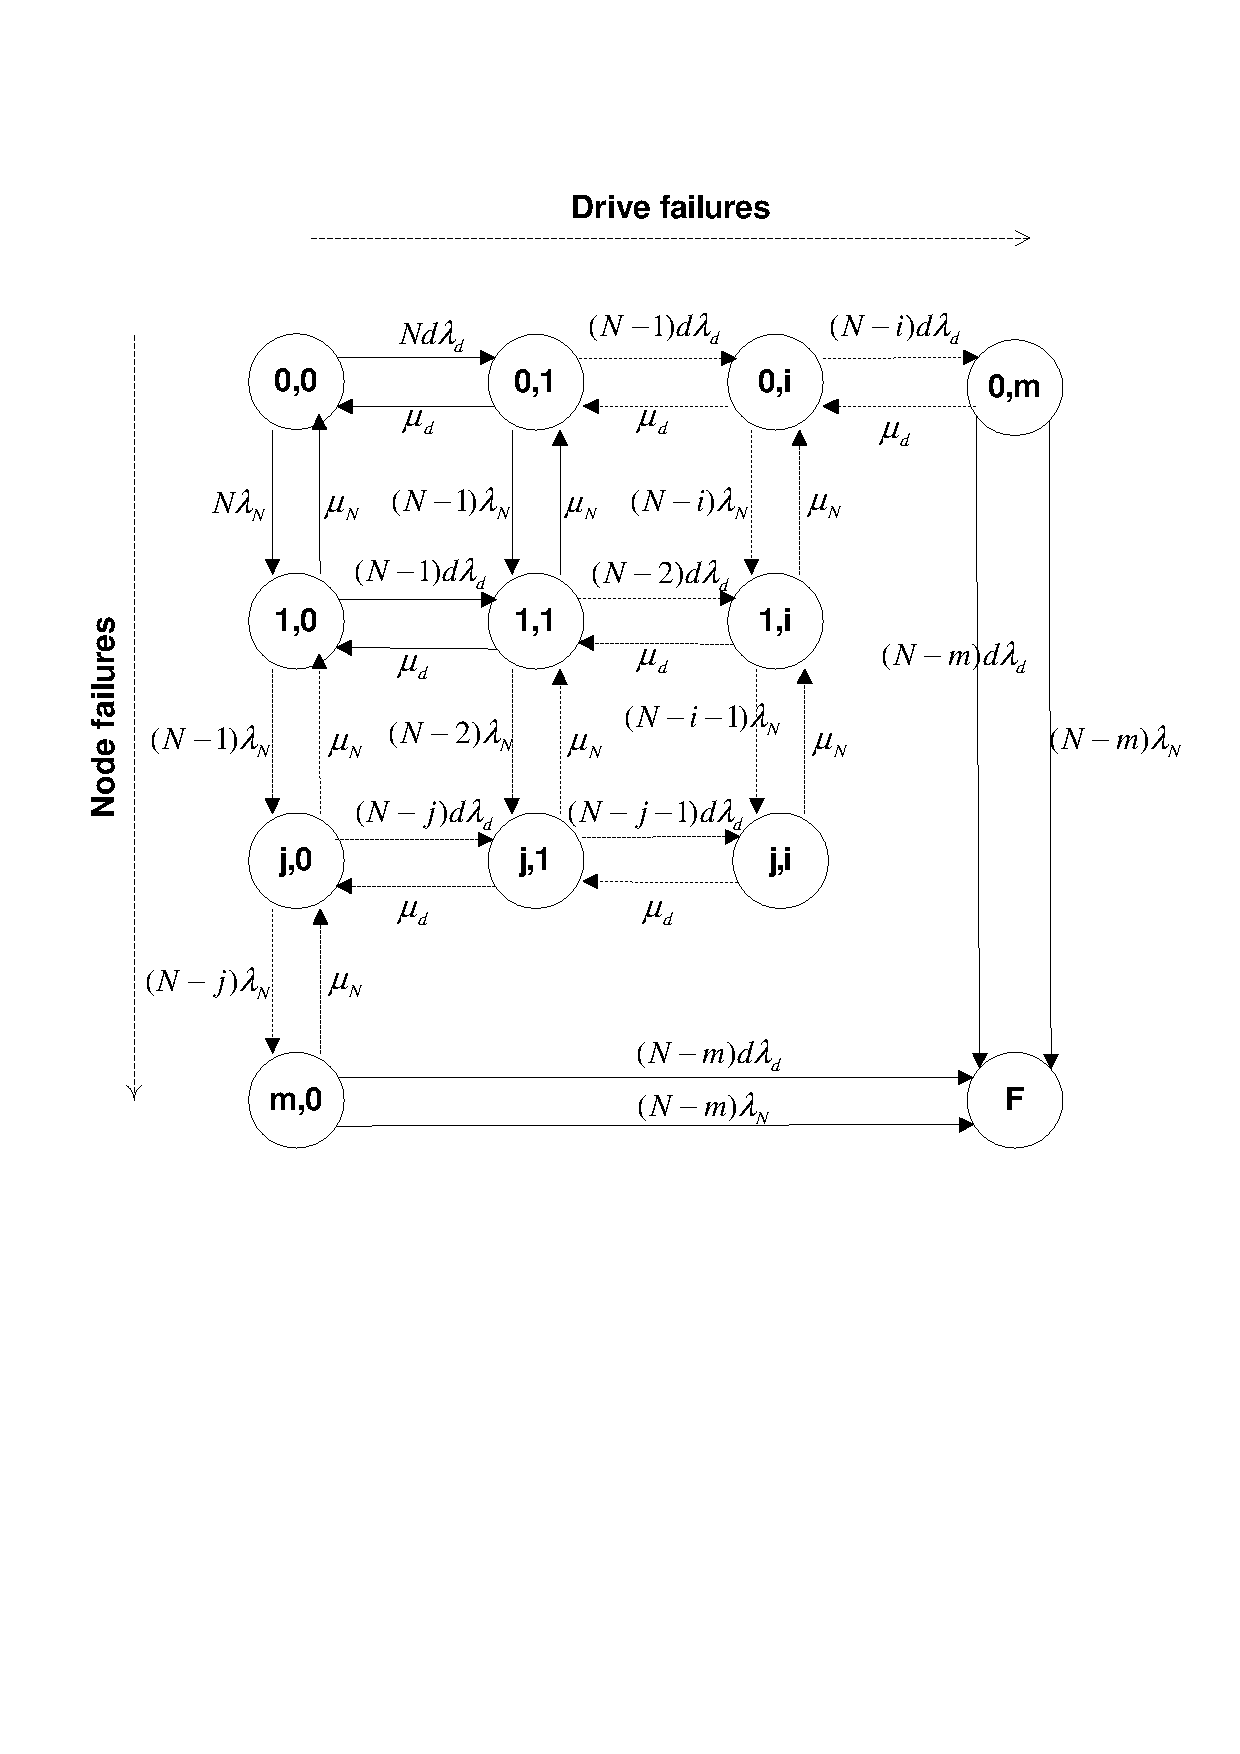
\includegraphics[width=\textwidth]{ClusterMarkov}
\end{center}
\caption{Markov Model for Clustered Storage}
\label{fig-markov-cluster}
\end{figure}

\begin{thebibliography}{99}

\bibitem{eval} R. Billinton and R.N. Allan. Reliability Evaluation of
Engineering Systems.  Plenum Press, New York and London, 1992.

\bibitem{markov} N.B. Fuqua.  The Applicability of Markov Analysis Methods to
Reliability, Maintainability, and Safety.  Selected Topics in Assurance
Related Technologies, volume~10, number~2.

\bibitem{google} S. Ghemawat, H. Gobioff, and S. Leung.  The Google File
System.  Symposium on Operating Systems Principles 2003.

\bibitem{chains} J.R. Norris. Markov Chains. Cambridge University Press, 1997.

\bibitem{raid} D.A. Patterson, G. Gibson, and R.H. Katz.  A Case for Redundant
Arrays of Inexpensive Disks (RAID).  Proc. Int'l Conf. Management of
Data, ACM, 1989, pp.~109-116.

\bibitem{plank} J. Plank. A Tutorial on Reed-Solomon Coding for
Fault-Tolerance in RAID-like Systems.  Available through
http://cs.utk.edu/~plank/, February 1999.

\bibitem{ibm} K.K. Rao, J.L. Hafner, R.A. Golding.  Reliability for Networked
Storage Nodes.  Technical Report RJ 10358, IBM Research, September~2005.

\bibitem{prob} S. Ross.  Introduction to Probability Models.  Academic Press;
7th edition, February 2000.

\bibitem{mss}
Q. Xin, et al.  Reliability Mechanisms for Very Large Storage Systems.  20th
IEEE / 11th NASA Goddard Conference on Mass Storage Systems and Technologies,
San Diego, CA, April 2003.

\end{thebibliography}

\end{document}
